\clearpage

\section{DISEÑO METODOLÓGICO}

El presente proyecto se desarrollará siguiendo un enfoque de ingeniería de 
software, orientado a la construcción de una plataforma que permita gestionar 
el ciclo operativo del Desafío Bebras en Bolivia. Para ello, se definirá una 
estrategia de trabajo estructurada que integre el análisis de requerimientos, 
el diseño de la solución, el desarrollo del sistema y su validación mediante 
pruebas.

\subsection{Arquitectura modular del sistema}

    La plataforma se implementará como un sistema web bajo una arquitectura
    cliente-servidor con un enfoque modular, en el cual el sistema se divide
    en componentes funcionales independientes que operan de manera integrada.
    Este enfoque facilita el desarrollo incremental, el mantenimiento y la
    escalabilidad del sistema, orientándolo a gestionar los procesos clave del
    concurso en el ámbito escolar boliviano. La Figura~\ref{fig:relacion-modulos}
    presenta de manera general la relación entre los cuatro módulos definidos
    para la plataforma. Los módulos principales que conforman el sistema se
    describen a continuación:

    \begin{figure}[H]
        \centering
        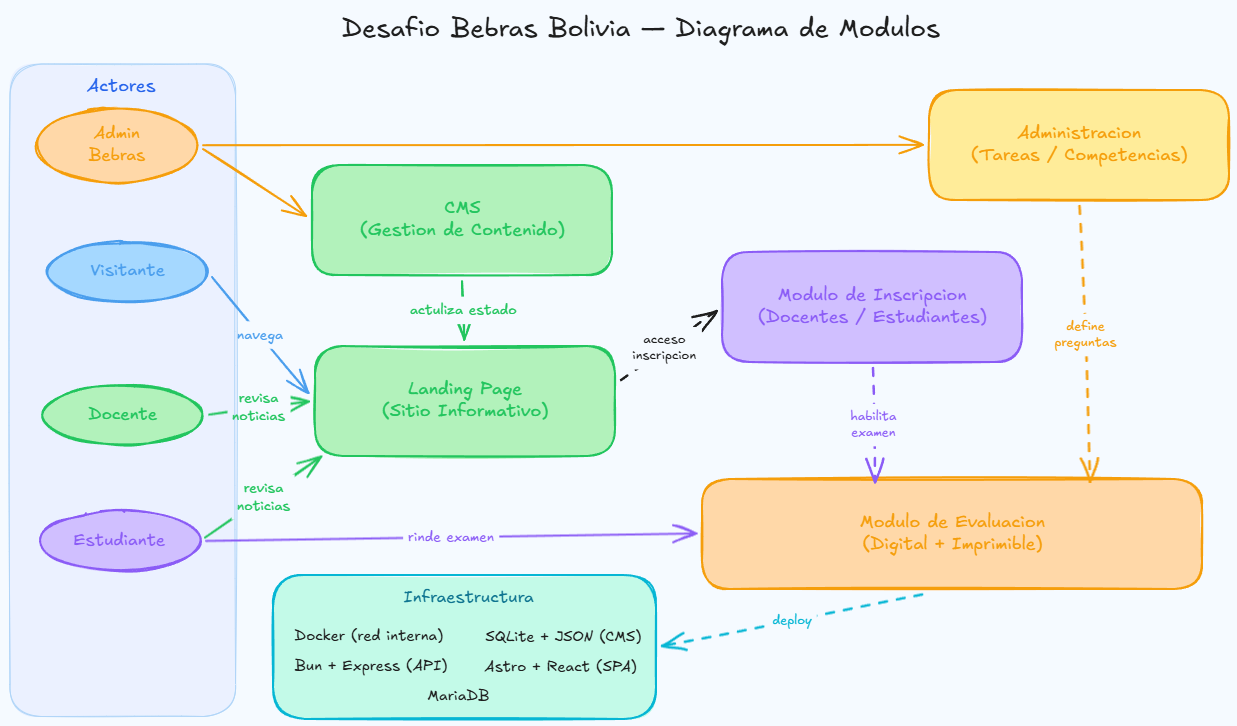
\includegraphics[width=0.8\textwidth]{assets/relacion_modulos.png}
        \caption{Relación entre los módulos principales de la plataforma}
        \label{fig:relacion-modulos}
    \end{figure}

    \begin{tikzpicture}[
    every node/.style={font=\small},
    actor/.style={
        ellipse, draw, thick, align=center,
        minimum width=2.4cm, minimum height=1.1cm
    },
    module/.style={
        rounded rectangle, draw, thick, align=center,
        minimum width=3.8cm, minimum height=1.3cm,
        rounded rectangle arc length=120
    },
    actor_admin/.style={actor, fill=orange!50, draw=orange!80},
    actor_visitor/.style={actor, fill=cyan!35, draw=cyan!60},
    actor_docente/.style={actor, fill=green!40, draw=green!65},
    actor_student/.style={actor, fill=violet!35, draw=violet!60},
    mod_cms/.style={module, fill=green!35, draw=green!65},
    mod_landing/.style={module, fill=green!35, draw=green!65},
    mod_admin/.style={module, fill=yellow!50, draw=yellow!75},
    mod_inscripcion/.style={module, fill=violet!30, draw=violet!55},
    mod_evaluacion/.style={
        module, fill=orange!40, draw=orange!70,
        minimum width=4.4cm
    },
    infra/.style={
        draw=cyan!55, fill=cyan!12, thick,
        rounded corners=10pt, align=center
    },
    solid/.style={-{Stealth[length=5pt]}, thick},
    dasharr/.style={-{Stealth[length=5pt]}, thick, dashed},
    lbl/.style={
        font=\scriptsize\itshape, fill=white,
        inner sep=2pt
    },
]

% ── Actores ────────────────────────────────────────────────────────────────
\node[actor_admin]   (admin)     at (0, 12.0) {Admin\\Bebras};
\node[actor_visitor] (visitante) at (0,  9.0) {Visitante};
\node[actor_docente] (docente)   at (0,  6.5) {Docente};
\node[actor_student] (student)   at (0,  3.5) {Estudiante};

\begin{scope}[on background layer]
  \node[
    draw=blue!35, fill=blue!8, thick,
    rounded corners=10pt,
    fit=(admin)(visitante)(docente)(student),
    inner sep=18pt,
    label={[blue!55, font=\small\itshape]above left:Actores}
  ] (actor_box) {};
\end{scope}

% ── Columna central ────────────────────────────────────────────────────────
\node[mod_cms]     (cms)     at (5.5, 12.0) {CMS\\(Gestión de Contenido)};
\node[mod_landing] (landing) at (5.5,  7.5) {Landing Page\\(Sitio Informativo)};

% ── Columna derecha ────────────────────────────────────────────────────────
\node[mod_admin]       (administracion) at (11.5, 12.0)
    {Administración\\(Tareas / Competencias)};
\node[mod_inscripcion] (inscripcion)    at (11.5,  9.0)
    {Módulo de Inscripción\\(Docentes / Estudiantes)};
\node[mod_evaluacion]  (evaluacion)     at (11.5,  5.0)
    {Módulo de Evaluación\\(Digital + Imprimible)};

% ── Infraestructura ────────────────────────────────────────────────────────
\node[infra, minimum width=10cm, minimum height=2.0cm]
    (infra) at (7.0, 1.2) {
        \textbf{Infraestructura}\\[4pt]
        Docker (red interna)\quad SQLite + JSON (CMS)\quad
        Bun + Express (API)\\
        Astro + React (SPA)\quad MariaDB
    };

% ══ FLECHAS ════════════════════════════════════════════════════════════════

% Admin → CMS (horizontal, fila 12)
\draw[solid, orange!80]
    (admin.east)
    -- node[lbl, above]{gestiona}
    (cms.west);

% CMS → Administración (horizontal, fila 12)
\draw[solid, orange!75]
    (cms.east)
    -- node[lbl, above]{actualiza config}
    (administracion.west);

% CMS → Landing (vertical bajada)
\draw[solid, green!60!black]
    (cms.south)
    -- node[lbl, right]{actualiza estado}
    (landing.north);

% Visitante → Landing (entra por oeste, y=8.2 → offset +0.7 arriba del centro)
\draw[solid, cyan!65!black]
    (visitante.east)
    -- node[lbl, above]{navega}
    ([yshift=8pt]landing.west);

% Docente → Landing (entra centrado en el oeste)
\draw[solid, green!65!black]
    (docente.east)
    -- node[lbl, above]{revisa noticias}
    (landing.west);

% Estudiante → Landing
% Sube desde y=3.5 hasta y=6.8, luego va horizontal al oeste de Landing
\draw[solid, violet!60]
    (student.east) -- ++(1.0, 0)
    -- ++(0, 3.8)
    -- node[lbl, above]{revisa noticias}
    ([yshift=-8pt]landing.west);

% Landing → Inscripción
\draw[dasharr, green!55!black]
    (landing.east)
    -- node[lbl, above]{acceso inscripción}
    (inscripcion.west);

% Administración → Inscripción (bajada directa)
\draw[dasharr, orange!70]
    (administracion.south)
    -- node[lbl, right]{define preguntas}
    (inscripcion.north);

% Inscripción → Evaluación (bajada directa)
\draw[dasharr, violet!55]
    (inscripcion.south)
    -- node[lbl, right]{habilita examen}
    (evaluacion.north);

% Estudiante → Evaluación
% Baja por el sur, viaja por debajo de todo, sube al sur de Evaluación
\draw[solid, violet!60]
    (student.south)
    -- ++(0, -1.5)                     % baja a y=2.0
    -- ++(12.8, 0)                     % cruza a x≈12.8, por debajo de infra
    -- node[lbl, right, pos=0.7]{rinde examen}
    (evaluacion.south);

% Evaluación → Infraestructura
\draw[dasharr, cyan!55!black]
    (evaluacion.south)
    -- ++(0, -0.5)
    -| node[lbl, above, pos=0.25]{deploy}
    (infra.east);

\end{tikzpicture}

    \begin{itemize}
        \item \textbf{Módulo de gestión de competencias y tareas:} permite la creación,
        categorización y administración de tareas de pensamiento computacional según
        rangos de edad escolar y niveles de dificultad, siguiendo los criterios
        establecidos por la organización internacional de Bebras.

        \item \textbf{Módulo de gestión de contenido institucional:} gestiona la información
        pública del Desafío Bebras Bolivia, permitiendo la administración dinámica de
        publicaciones, noticias y estructura del sitio web informativo orientado a
        docentes e instituciones escolares.

        \item \textbf{Módulo de registro y administración de participantes escolares:} gestiona
        la inscripción y administración de unidades educativas de nivel primario y
        secundario, docentes responsables y estudiantes participantes, organizando su
        participación según las categorías del concurso.

        \item \textbf{Módulo de evaluación digital e imprimible:} soporta la resolución de
        tareas en entorno web y la generación de formatos imprimibles para su
        procesamiento mediante reconocimiento óptico de caracteres, adaptados a las
        condiciones de conectividad de unidades educativas escolares bolivianas.
    \end{itemize}

\subsection{Metodología de desarrollo}

    El desarrollo de la plataforma se realizará mediante la metodología ágil
    Extreme Programming (XP), dado que resulta particularmente adecuada para
    equipos pequeños como el presente proyecto, conformado por dos desarrolladores.
    XP prescinde de los roles formales propios de marcos más extensos y privilegia
    prácticas como la programación en pareja, la integración continua, el diseño
    simple, el refactorizado progresivo y las iteraciones cortas, lo que permite
    adaptarse con flexibilidad a cambios en los requerimientos y mantener un ritmo
    sostenible de trabajo \cite{beckandres2004}.

    En este marco, el trabajo se organizará en iteraciones cortas orientadas a la
    construcción de incrementos funcionales de la plataforma. Cada iteración tendrá
    una duración aproximada de dos semanas y estará sujeta a revisión continua,
    incorporando retroalimentación directa de los usuarios vinculados al concurso
    \cite{beckandres2004}. El proceso de desarrollo se estructura en las siguientes
    etapas:

    \begin{itemize}
        \item \textbf{Análisis:} identificación de requerimientos y estudio de los
        procesos organizativos del Desafío Bebras aplicados al contexto escolar
        boliviano.

        \item \textbf{Diseño:} definición de la arquitectura del sistema, modelado
        de la base de datos y diseño de módulos.

        \item \textbf{Desarrollo:} implementación progresiva de los módulos definidos,
        aplicando programación en pareja e integración continua.

        \item \textbf{Pruebas:} evaluación del sistema mediante pruebas funcionales
        con usuarios vinculados al concurso.
    \end{itemize}

\subsection{Herramientas y tecnologías}

    Para el desarrollo e implementación de la plataforma se empleará el siguiente
    conjunto de herramientas y tecnologías:

    \begin{itemize}
        \item \textbf{Backend:} Bun, Express.
        \item \textbf{Frontend:} Astro, React.
        \item \textbf{Base de datos:} MariaDB, SQLite.
        \item \textbf{Almacenamiento de contenido:} archivos JSON.
        \item \textbf{Contenedores:} Docker.
        \item \textbf{Control de versiones:} Git, GitHub.
        \item \textbf{Entorno de desarrollo:} Visual Studio Code.
    \end{itemize}

\subsection{Cronograma}

    Para la organización de las actividades del proyecto se ha definido un cronograma
    de trabajo que estructura las tareas en función de los objetivos específicos
    planteados y de los módulos que conforman el sistema.

    Las actividades 1 y 2 corresponden a la fase de análisis, orientada a la
    identificación de los procesos organizativos del Desafío Bebras y a la
    consolidación de los requerimientos del sistema. Las actividades 3 y 4
    conforman la fase de diseño, abordando la arquitectura modular, el modelo
    de datos y la estrategia de despliegue.

    Las iteraciones de desarrollo (actividades 5 a 8) están alineadas directamente
    con los módulos del sistema: la Iteración 1 (actividad 5) implementa el módulo
    de gestión de contenido institucional (CMS) y el sitio web informativo;
    la Iteración 2 (actividad 6) desarrolla el módulo de gestión de competencias
    y tareas; la Iteración 3 (actividad 7) construye el módulo de registro y
    administración de participantes escolares; y la Iteración 4 (actividad 8)
    implementa el módulo de evaluación digital e imprimible. Durante cada una
    de estas iteraciones, en paralelo al incremento funcional correspondiente,
    se avanzará la documentación del sistema, de modo que esta no quede
    concentrada al final del proyecto.

    Las actividades 9 y 10 integran los módulos desarrollados, aplican la
    contenerización del sistema y verifican su comportamiento mediante pruebas
    funcionales en entorno controlado. Finalmente, las actividades 11 y 12 se
    dedican al refinamiento y estructuración formal del documento ya redactado
    a lo largo de las iteraciones, y a los ajustes finales previos a la defensa
    del proyecto.

    El detalle de las actividades, recursos y resultados esperados se presenta
    en la Tabla~\ref{tab:cronograma}.

    \begin{table}[H]
    \centering
    \caption{Cronograma de actividades}
    \label{tab:cronograma}
    \small
    \begin{tabular}{|c|p{3.5cm}|c|c|p{3cm}|p{3.5cm}|}
    \hline
    \textbf{Nro.} & \textbf{Actividad} & \textbf{Inicio} & \textbf{Fin} & 
    \textbf{Recursos} & \textbf{Resultados} \\
    \hline
    1 & Analizar procesos organizativos del Desafío Bebras y requerimientos del contexto escolar boliviano &
    01/03/2026 & 08/03/2026 &
    Documentación internacional Bebras, entrevistas, observación &
    Mapa de procesos y catálogo inicial de requerimientos \\
    \hline
    2 & Analizar experiencias de países miembros & 
    08/03/2026 & 15/03/2026 & 
    Plataformas Bebras, documentación técnica & 
    Requerimientos funcionales consolidados \\
    \hline
    3 & Diseñar arquitectura modular y despliegue en contenedores & 
    15/03/2026 & 30/03/2026 & 
    Visual Studio Code, Docker, diagramas & 
    Arquitectura definida, comunicación entre servicios y estrategia de despliegue \\
    \hline
    4 & Diseñar modelo de datos y almacenamiento &
    30/03/2026 & 06/04/2026 &
    MariaDB, SQLite, diagramas &
    Modelo de datos y estrategia híbrida de almacenamiento \\
    \hline
    5 & Iteración 1: Módulo CMS (sitio estático) &
    06/04/2026 & 27/04/2026 &
    Astro, React, SQLite, JSON, Git &
    CMS funcional, sitio informativo desplegable y avance de la documentación \\
    \hline
    6 & Iteración 2: Módulo de competencias &
    28/04/2026 & 11/05/2026 &
    Astro, React (SPA), Bun, Express, MariaDB &
    Gestión de tareas, lógica base de competencias y avance de la documentación \\
    \hline
    7 & Iteración 3: Registro de participantes &
    12/05/2026 & 24/06/2026 &
    Astro, React (SPA), Bun, Express, MariaDB &
    Sistema de inscripción, administración de usuarios y avance de la documentación \\
    \hline
    8 & Iteración 4: Evaluación digital &
    25/06/2026 & 09/07/2026 &
    Astro, React (SPA), Bun, Express, MariaDB &
    Ejecución de pruebas, generación de evaluaciones y avance de la documentación \\
    \hline
    9 & Integración y contenerización del sistema &
    10/07/2026 & 19/07/2026 &
    Docker, configuración de red &
    Sistema integrado en contenedores y listo para validación \\
    \hline
    10 & Pruebas funcionales del sistema &
    20/07/2026 & 30/07/2026 &
    Casos de prueba, usuarios vinculados al concurso &
    Validación funcional del sistema en entorno controlado \\
    \hline
    11 & Refinamiento y estructuración formal del documento &
    31/07/2026 & 14/08/2026 &
    \LaTeX, GitHub &
    Documento técnico con estructura y formato finales, a partir del borrador avanzado durante los sprints \\
    \hline
    12 & Ajustes finales y defensa & 
    15/08/2026 & 29/08/2026 & 
    Sistema completo & 
    Versión final del sistema y presentación \\
    \hline
    \end{tabular}
\end{table}